\documentclass{beamer}
\usepackage[utf8]{inputenc}
\usepackage[french]{babel}
\usepackage{graphics}
\usepackage{multirow}
\usepackage{colortbl}
\usepackage{CJKutf8}

%\usepackage[screen,nopanel]{pdfscreen}
%\usepackage{url}

\usetheme{metropolis}

\title{Projet agile N3}
\author{
  %\includegraphics[width=3cm]{logo_azae.png}
}
  
\date{}

\logo{
  \raisebox{-0.5\height}{\includegraphics[width=1cm]{cc_by_sa} }
}


\begin{document}

\frame{\titlepage}

\begin{frame}{C'est quoi ?}
 
  {\Large \alert{Être agile} et pas faire de l'Agile.}

  \vspace{6mm}
  C'est avant tout un état d'esprit partagé par l'ensemble des participants à un projet.
\end{frame}

\begin{frame}{Être agile}
  "Les firmes qui survivent dans le long terme ne sont pas celles qui sont les plus fortes ou les plus intelligentes, mais celles qui s'adaptent le mieux aux changements d'environnement"

  \flushright{Hiroshi Okuda, Toyota}

\end{frame}

\begin{frame}{Le manifeste agile}
  \large
  \alert{Individuals and interactions} over processes and tools\newline
  \alert{Working software} over comprehensive documentation\newline
  \alert{Customer collaboration} over contract negotiation\newline
  \alert{Responding to change} over following a plan
\end{frame}

\begin{frame}{Valeurs et principes}
  \Large Des cycles courts, un produit en production à chaque fin de cycle et des producteurs de valeurs qui s'améliorent continuellement.
\end{frame}

\begin{frame}{Le radiateur d'information}
  \begin{itemize}
    \item Donner les moyens aux acteurs d'être autonomes
    \item Faire rayonner l'information
    
    \begin{itemize}
      \item Vision du projet, Proposition de valeur unique
      \item Date de livraison, avancement, etc.
      \item Planning des congés
      \item Actions d'améliorations
      \item Backlog
      \item Problèmes
      \item Etc.
    \end{itemize}
  \end{itemize}
\end{frame}

\begin{frame}{Exemple de radiateur}
  \center
  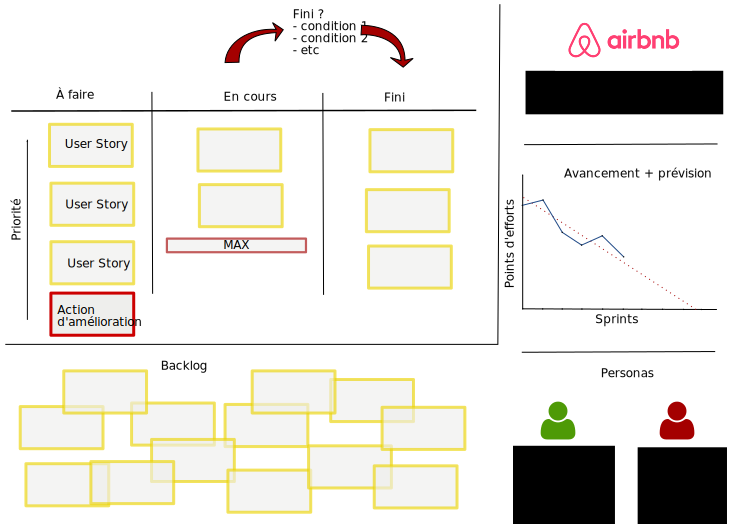
\includegraphics[width=10cm]{includes/radiateur}
\end{frame}

\begin{frame}{Kaizen 
    {\begin{CJK*}{UTF8}{mj} 改善 \end{CJK*}}
  }
  \center
  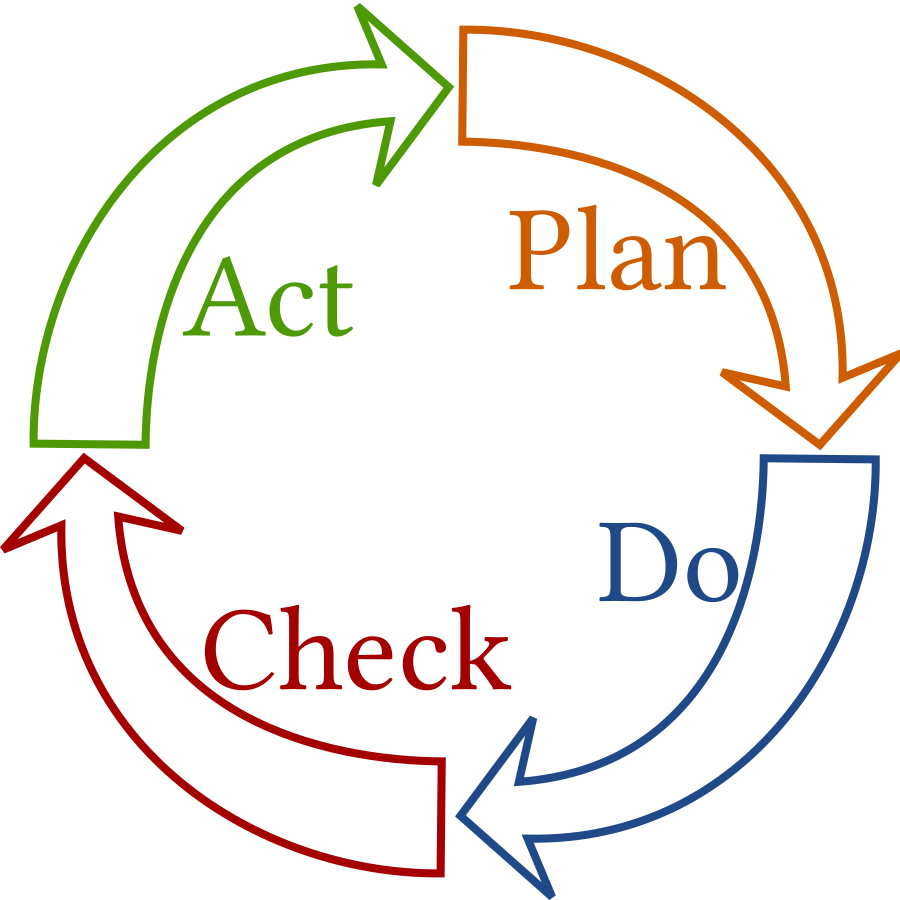
\includegraphics[width=6cm]{includes/pdca}
\end{frame}

\begin{frame}{Kaizen 
    {\begin{CJK*}{UTF8}{mj} 改善 \end{CJK*}}
  }
  
  \begin{itemize}
    \item \alert{Plan} : Identifier une action d'amélioration et un élément observable qui pourra permettre de déterminer si l'action à porté ses fruits ou pas.
    \item \alert{Do} : Faire l'action sur un temps donné, une itération par exemple.
    \item \alert{Check} : Prendre le temps de mesurer si l'action a apporté le changement souhaité
    \item \alert{Act} : Décider, l'action est peut-être à répéter, une autre action peut en découler, etc.
  \end{itemize}

\end{frame}

\newcolumntype{g}{>{\columncolor[gray]{0.8}}c}

\begin{frame}{Planning de la semaine}{}
  {
    \center
    \begin{tabular}{l | g | g | g  }
      & \textbf{06/06} & \textbf{07/06} & \textbf{08/06} \\
      \hline
      08h00 - 10h00 & Théorie & Sprint & Sprint \\
      \hline
      10h00 - 12h00 & Sprint 0 & Sprint & Sprint \\
      \hline
      13h30 - 15h30 & Sprint & Sprint & Restitution \\
      \hline
      15h30 - 17h30 & Sprint & Sprint & Rétrospective \\
      \hline
    \end{tabular}
  }

\end{frame}

\begin{frame}{Un Sprint}
  \begin{itemize}
    \item 1,5h de production
    \item 30 minutes pour améliorer la capacité de production
    \begin{itemize}
      \item Démo d'équipe
      \item Rétrospective d'équipe
      \item Action d'amélioration
    \end{itemize}
    \item 1,5h de production
    \item 30 minutes pour améliorer la capacité de production
    \begin{itemize}
      \item Démo de groupe
      \item Rétrospective de groupe
      \item Action d'amélioration
      \item Pause
    \end{itemize}
  \end{itemize}
\end{frame}

\begin{frame}{Détail du Sprint 0}
  Une après midi, 4 Objectifs : 
  \begin{itemize}
    \item Partager la vision du produit
    \item Découper et estimer le backlog
    \item Construire la proposition de valeur unique :
    \begin{itemize}
      \item Cible
      \item Problème
      \item Solution
    \end{itemize}
    \item Initier la pile technique et montrer que l'on est capable de livrer de la valeur.
  \end{itemize}
\end{frame}

\begin{frame}{Restitution}
  Vous devez convaincre que le travail réalisé durant les 3 jours était extraordinaire.
  \begin{itemize}
    \item Montrez nous le résultat
    \item Expliquez ce que vous avez appris
  \end{itemize}
\end{frame}

\begin{frame}{Contraintes}
  \begin{itemize}
    \item Du java
    \item pas d'IHM swing temps qu'il n'existe pas une IHM texte
  \end{itemize}
\end{frame}

\end{document}

